\subsection{Simulação 2 - Simulação completa}

Após a avaliação das extremidades da pá, deve-se ainda simular o revestimento
total, pois a superfície da pá é muito irregular, podendo se aproximar ou se
afastar do robô para certas posições de base. Além disso, foram abordadas novas
estratégias para a solução de revestimento da extremidade direita da pá. A
simulação de teste de toda a pá considerou as seguintes variáveis:

\begin{itemize}
  \item O ângulo das pás da turbina variam de $0^o a 24^o$. O acréscimo deste
  grau de liberdade buscou solucionar o problema da extremidade direita.
  \item O rotor da turbina foi girado de $0^o$ a $30^o$ com passo de $3^o$.
  Manteve-se este grau de liberdade, pois em conjunto com o giro da pá, o
  problema da extremidade superior direita poderia ser solucionado.
  \item A distância entre extremidade da pistola e pá pode variar $235
  \pm 5$ mm.
  \item O ângulo entre a pistola e o plano da pá pode variar $90^o \pm
  30^o$. Alguns testes utilizaram a tolerância limite de $60^o$ como tentativa
  de revestir a extremidade direita superior.
  \item A posição em $y$ do robô foi mantida fixa. $-3220$ mm na referência
  global.
  \item A posição em $x$ do robô foi mantida fixa. $1200$ mm de
  distância em relação a pá.
  \item A posição em $z$ do robô foi amostrada uniformemente em 10 pontos ao
  longo da pá. A equipe de mecânica restringiu o movimento em $z$ tal que
  $-1240 < z < 1240$, garantindo para este $y$ mínimo ($-3220$ mm) espaço
  suficiente para a construção do trilho.
\end{itemize}

A partir dos parâmetros dados, foram realizadas as seguintes simulações:
\begin{enumerate}
  \item Variação da base apenas em $z$, variação do ângulo do rotor e do ângulo
  da pá.
  \item Variação de tolerância do ângulo entre pistola de revestimento e pá: $90^o \pm
  60^o$.
  \item Variação do rotor e ângulo da pá.
\end{enumerate}

\subsubsection{Teste completo - 1 }\label{teste1}

A restrição da mecânica para a construção do trilho $-1240$ mm $< z <$ $1240$ mm
prejudica o revestimento na lateral direita da pá, região em que o aro câmara
está próximo de $20^o$. A figura~\ref{fig::simcomp1_1} mostra a
discretização completa da pá, nas condições em que o rotor está $0^o$ e a pá
$24^o$:
em preto, pontos revestidos; e em vermelho, pontos que não foram revestidos para
esta posição do robô. Como pode ser visto, não foi possível revestir a pontos da
lateral direita, a extremidade superior direita e a extremidade superior
esquerda.

\begin{figure}[!ht]
	\centering	
	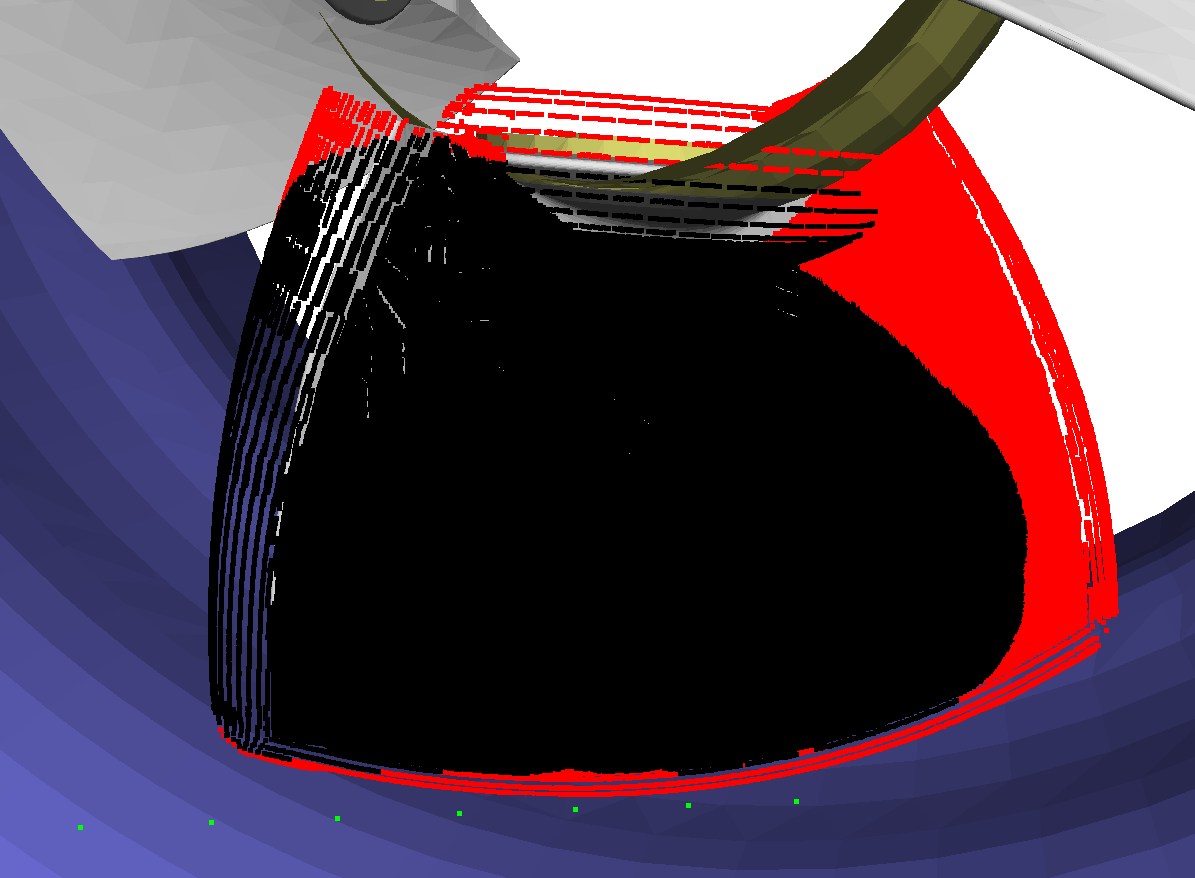
\includegraphics[width=.5\columnwidth]{figs/simcomp1_1.png}
	\caption{Simulação de revestimento completo da pá, considerando as
	restrições mecânicas da base, ângulo $0^o$ do rotor e $24^o$ da pá.}
	\label{fig::simcomp1_1}
\end{figure}

A extremidade superior esquerda só será revestida caso haja elevação da base do
robô ou, talvez, utilizando tolerância de ângulo de revestimento $60^o$.
Como esta região da pá tem inclinação, estando projetada para o robô, alterar
o ângulo da pá para $0^o$ não favorece o revestimento. 

Em relação à lateral direita da pá, a ideia imediata é rotar a turbina,
esperando que o lado direito se aproxime do robô. Outra possibilidade é girar a
pá em seu próprio eixo para $0^o$, em vez de $24^o$. 

A figura~\ref{fig::simcomp1_2} mostra a discretização completa da pá, nas
condições em que o rotor está $15^o$ e a pá $24^o$: em preto, pontos
revestidos; e em vermelho, pontos que não foram revestidos para esta posição do
robô. Conforme o rotor é girado, embora o revestimento aumente na lateral
direita da pá, a lateral esquerda e as áreas inferiores começam a não ser
revestidas. A extremidade superior direita continua sem ser revestida, como
esperado, vide subseção \ref{superioresquerda}. 

\begin{figure}[!ht]
	\centering	
	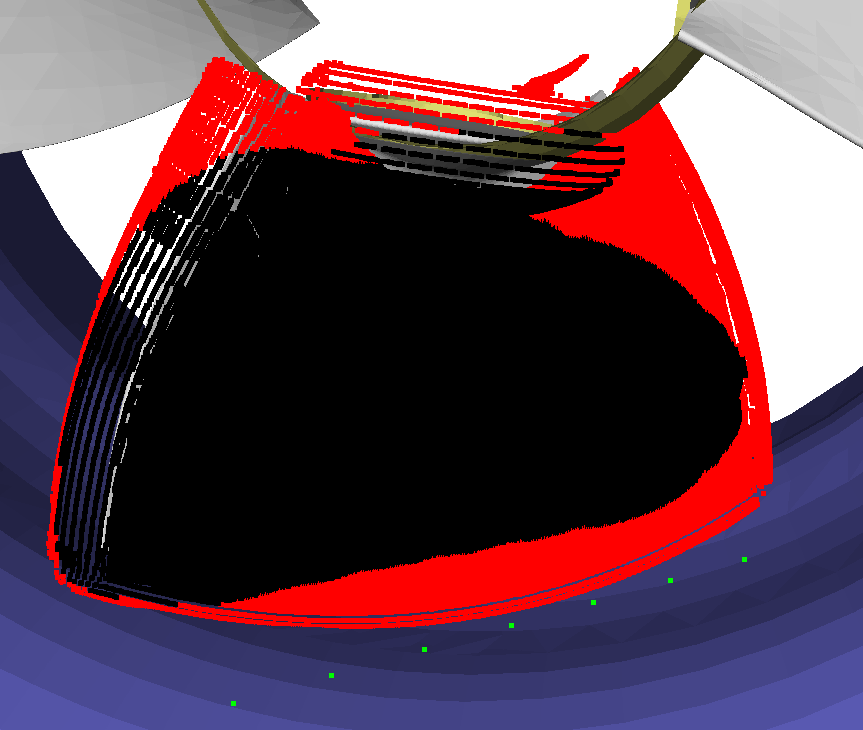
\includegraphics[width=.5\columnwidth]{figs/simcomp1_2.png}
	\caption{Simulação de revestimento completo da pá, considerando as
	restrições mecânicas da base, ângulo $15^o$ do rotor e $24^o$ da pá.}
	\label{fig::simcomp1_2}
\end{figure}

A figura~\ref{fig::simcomp1_4} mostra a discretização completa da pá, nas
condições em que o rotor está $0^o$ e a pá $0^o$: em preto, pontos
revestidos; e em vermelho, pontos que não foram revestidos para esta posição do
robô. Conforme a pá é girada, o revestimento aumenta na lateral direita e se
mantém na lateral direita. Isso ocorre, pois o robô se mantém longe do aro
câmara no lado direito, já que o aro ainda não está $20^o$. Esta é a melhor
posição para revestimento da pá, situação aparente ao método da Rijeza, porém a
extremidade superior direita ainda não foi revestida.

\begin{figure}[!ht]
	\centering	
	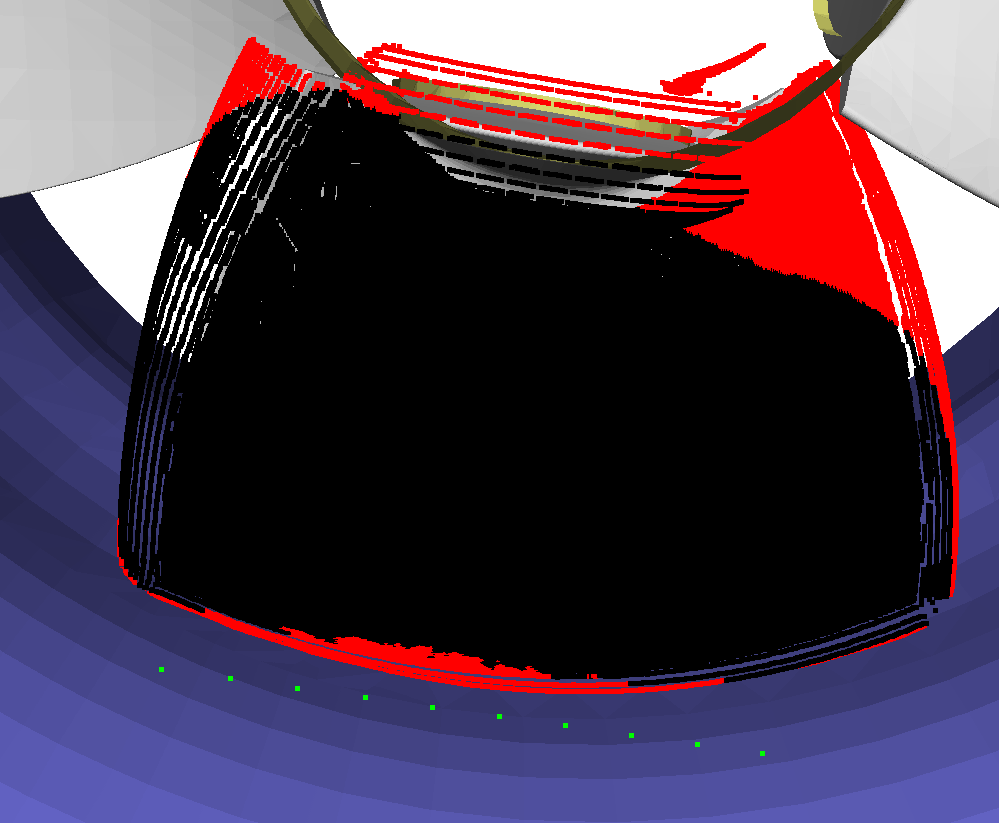
\includegraphics[width=.5\columnwidth]{figs/simcomp1_4.png}
	\caption{Simulação de revestimento completo da pá, considerando as
	restrições mecânicas da base, ângulo $0^o$ do rotor e $0^o$ da pá.}
	\label{fig::simcomp1_4}
\end{figure}

\subsubsection{Teste completo - 2}

Foi observado na subseção~\ref{teste1} que a extremidade superior esquerda não
foi revestida, podendo ser necessário  Quando aumentamos a tolerância de ângulo
de revestimento para $60^o$, obtemos a figura\ref{fig::simcomp1_3}. A figura mostra que foi possível revestir toda a
extremidade superior esquerda, salvo pontos de colisão com o rotor. Entretanto,
é importante a base ter o grau de liberdade em $y$ para eventuais problemas
suprir eventuais problemas de modelagem.

\begin{figure}[!ht]
	\centering	
	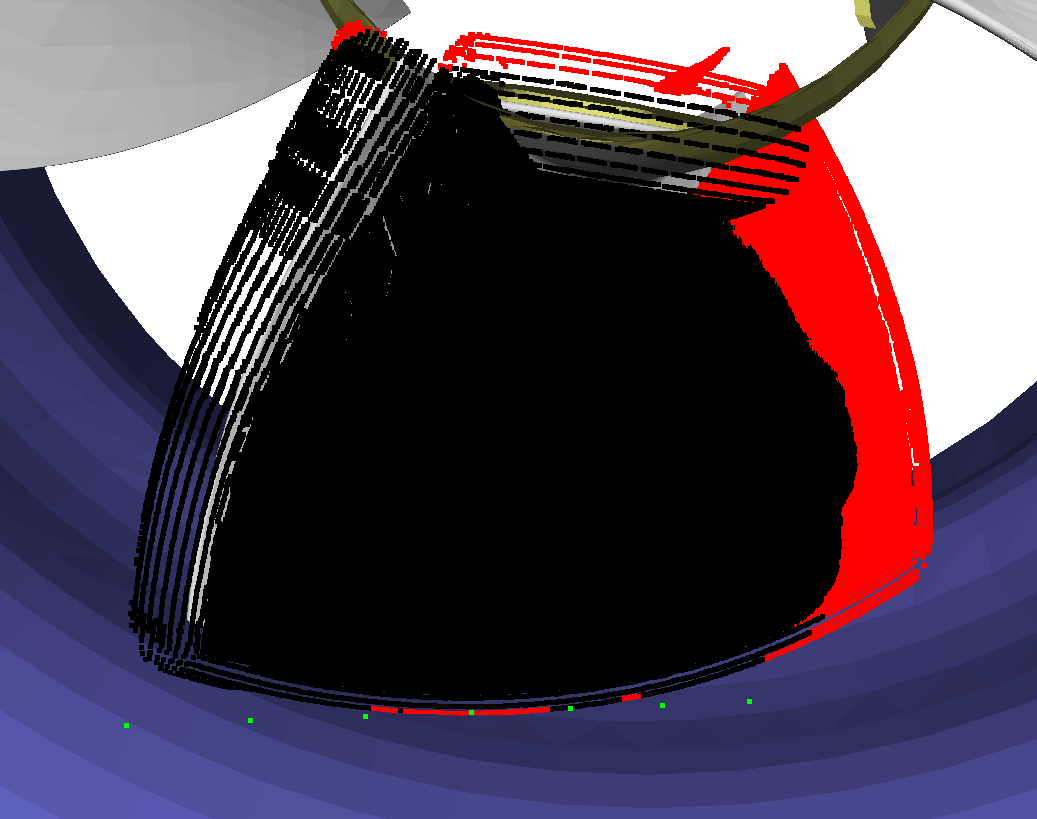
\includegraphics[width=.5\columnwidth]{figs/simcomp1_3.png}
	\caption{Simulação de revestimento completo da pá, considerando as
	restrições mecânicas da base, ângulo $0^o$ do rotor e $24^o$ da pá,
	tolerância de $60^o$ de revestimento.}
	\label{fig::simcomp1_3}
\end{figure}

\subsubsection{Extremidade superior esquerda}

A extremidade superior esquerda possui complexidade de posição do ponto a
ser revestido devido à altura do robô. A figura~\ref{fig::shoulderleft} mostra
a discretização da pá na extremidade esquerda: pontos azuis são pontos revestidos na tolerância de
$30^o$; em preto, pontos revestidos sem tolerância; e em vermelho, pontos que
não foram revestidos para esta posição do robô.

\begin{figure}[!ht]
	\centering	
	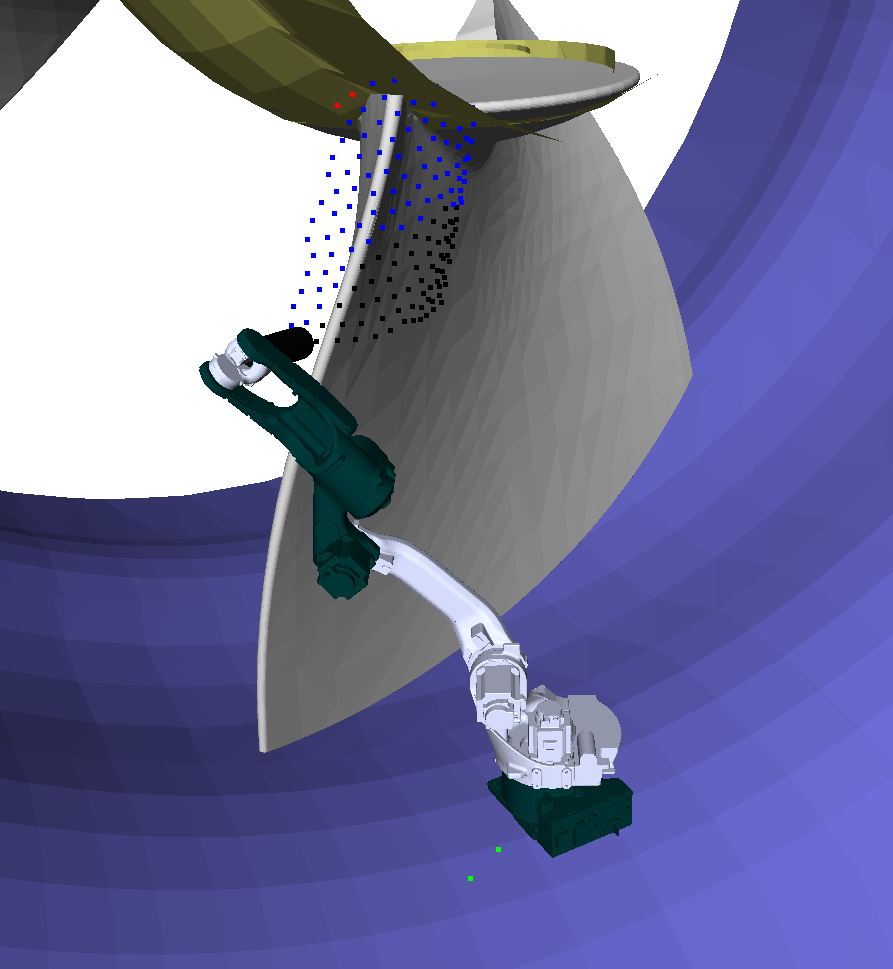
\includegraphics[width=.5\columnwidth]{figs/shoulderleft.png}
	\caption{Estudo de revestimento para a extremidade superior esquerda.}
	\label{fig::shoulderleft}
\end{figure}

A simulação mostrou que se mantivermos a altura da base em $y=-3220$ mm
(altura mínima) e $x=1300$ mm, são necessárias duas posições em $z$ (ao longo do
trilho) para o revestimento completo da extremidade. É interessante para o
projeto manter altura fixa o quanto possível, pois há redução de grau de
liberdade, e, portanto, redução na complexidade da base mecânica.

Caso haja alteração na altura do robô, por exemplo  $y=-2770$ mm, só será
necessária uma posição em $z$ para a conertura completa da região. Mas é
preferível mover o robô no trilho, em $z$, a mover o robô em altura, em $y$. 

A extremidade superior esquerda necessitou duas posições para a base, mas não
mostrou desafios técnicos.

\subsubsection{Extremidade superior direita}

A extremidade superior esquerda possui duas complexidades de revestimento:
posição do ponto devido à altura do robô; e vetor normal, direção de
revestimento. A figura~\ref{fig::shoulderright} mostra a discretização da pá na
extremidade esquerda: pontos azuis são pontos revestidos na tolerância de $30^o$; em preto, pontos revestidos sem tolerância; e em vermelho, pontos que
não foram revestidos para esta posição do robô.

\begin{figure}[!ht]
	\centering	
	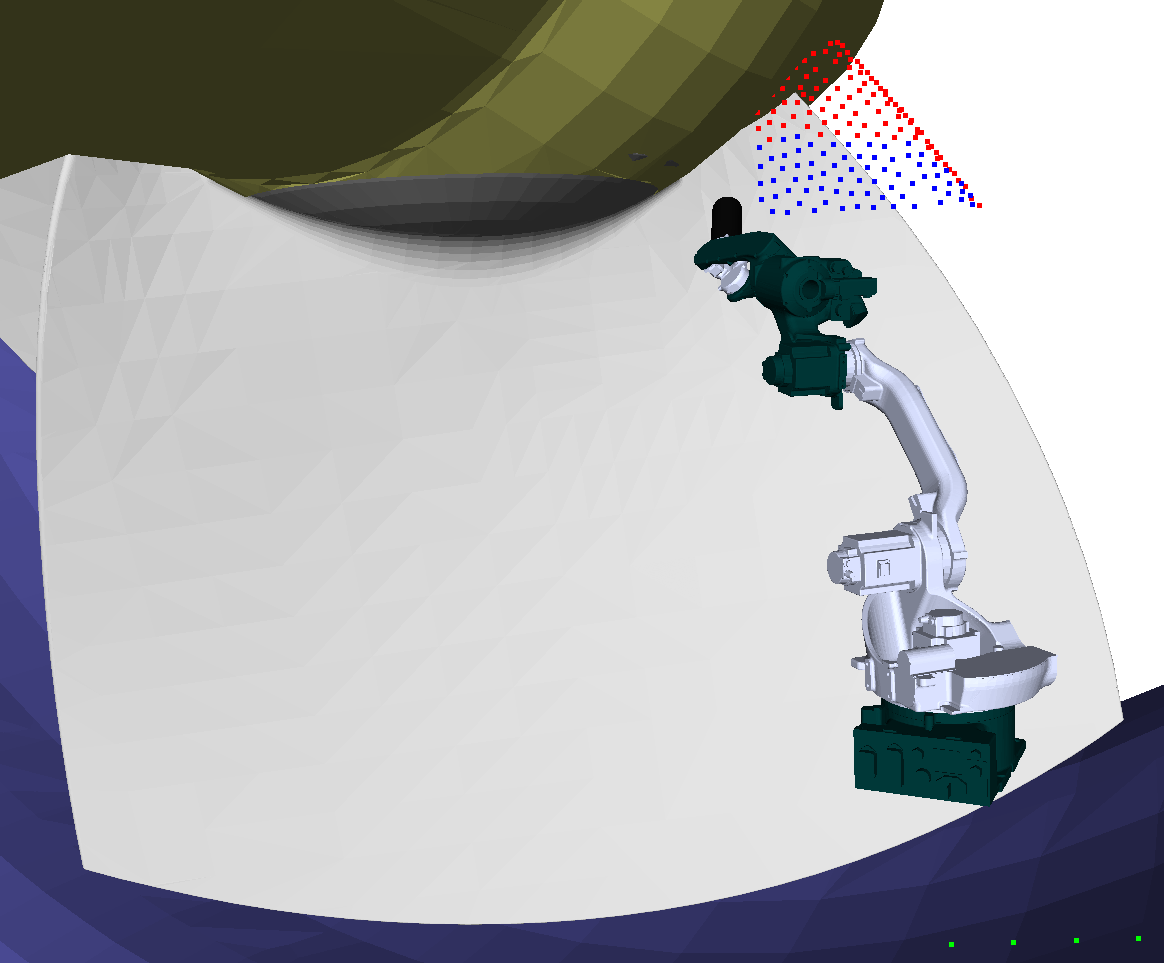
\includegraphics[width=.5\columnwidth]{figs/shoulderright.png}
	\caption{Estudo de revestimento para a extremidade superior direita.}
	\label{fig::shoulderright}
\end{figure}

A simulação mostra que, mesmo se utilizarmos a altura máxima para a base
$y=-2720$ mm e mantivermos $x=1300$ mm, não há posição em $z$ (ao longo do
trilho) para revestir por completo a extremidade. Aproximando o manipulador da
pá, novos pontos são revestido, mas mesmo em $x=230$ mm o
revestimento não é completo. O mesmo teste foi feito para diferentes
ângulos do rotor, mas os resultados não são favoráveis, pois conforme o rotor
gira, a pá se afasta do robô.

Para $y=-3220$ mm e $x=1300$ mm, nenhum ponto da extremidade superior direita é
revestido, logo outras estratégias devem ser adotadas. A extremidade superior
direita mostrou grande complexidade técnica e não foi possível encontrar uma
solução viável para o 2º trilho a fim de revestí-la.